\section{Theory}
\label{sec:theory}

The residual of the eikonal equation in a 2D domain ($\Omega$) can be written as
\begin{equation}
    \label{eqn:eik_res}
    r(\boldsymbol{x}):= \sqrt{\nabla T(\boldsymbol{x})\cdot\nabla T(\boldsymbol{x} )}-S(\boldsymbol{x}) = 0, \quad \boldsymbol{x} \in \Omega, 
\end{equation}
where $S(\boldsymbol{x})$ is the slowness which is the reciprocal of the velocity field $V(\boldsymbol{x})$. 

I use two separate ANNs composed of non-linear functions to approximate traveltimes $T(\boldsymbol{x})$ and velocities $V(\boldsymbol{x})$ in the eikonal equation, such that
\begin{equation}
\begin{aligned}
    \label{eqn:network_approx}
     \tilde{T}(\boldsymbol{x}) = \mathcal{N_{T}}(x_{s},\boldsymbol{x};w_{T},b_{T}), \\
     \tilde{V}(\boldsymbol{x}) = \mathcal{N_{V}}(\boldsymbol{x};w_{V},b_{V}),
\end{aligned}     
\end{equation}

where $\mathcal{N_{T}}$ and $\mathcal{N_{V}}$ are the feed-forward neural networks for traveltime and velocity respectively. Here the trainable parameters are weights and biases shown as $w_{T}$ and $b_{T}$ for traveltime NN and $w_{V}$ and $b_{V}$ for velocity NN. To honor multiple shots on the surface, horizontal coordinates of the source location denoted as $x_{s}$, are used as an additional input to the traveltime network, contrary to the velocity network. 

For stability as well as ensuring the solutions remain positive, sigmoid activation function $\sigma$ is applied for both output of the networks before multiplying them with the maximum expected velocity and traveltime values
\begin{equation}
\begin{aligned}
    \label{eqn:network_approx_sigmoid}
     \tilde{T}(\boldsymbol{x}) = T_{max}\,\, \sigma(\mathcal{N_{T}}(x_{s},\boldsymbol{x};w_{T},b_{T})), \\
     \tilde{V}(\boldsymbol{x}) = V_{max}\,\, \sigma(\mathcal{N_{V}}(\boldsymbol{x};w_{V},b_{V})),
\end{aligned}     
\end{equation}

where $V_{max}$ can be decided considering geology of the medium. Whereas, $T_{max}$ can easily be obtained from the observed times. The same strategy for constraining the PINN solution as strictly positive was previously used for prediction of activation maps in cardiac electrophysiology~\cite{cyphk:20}. Recovering the possible sharp transitions in the velocity solution, I also add isotropic total variation regularizer (TV) to the problem. Thus, the composite loss function to train both networks concurrently reads 

\begin{equation}
\begin{aligned}
    \label{eqn:loss}
     \mathcal{L}(w_{T},b_{T},w_{V},b_{V}) = \frac{1}{N_{S} N_{T}} \sum\limits_{n=1}^{N_{S}} \sum\limits_{i=1}^{N_{T}} (\tilde{T}(\boldsymbol{x}_{n,i}) - T_{n,i})^2 \\ + \frac{1}{N_{S} N_{C}} \sum\limits_{n=1}^{N_{S}} \sum\limits_{i=1}^{N_{C}}(\sqrt{\nabla\tilde{T}(\boldsymbol{x}_{n,i}) \cdot\nabla\tilde{T}(\boldsymbol{x}_{n,i})} - \tilde{S}(\boldsymbol{x}_{n,i}))^2 \\ +
     \lambda \frac{1}{N_{C}}\sum\limits_{i=1}^{N_{C}}\norm{\nabla\tilde{V}\boldsymbol({x}_{i})}.
\end{aligned}     
\end{equation}

The first term measures the misfit between the observed traveltimes and the network predicted ones on the receiver positions for each source location. $N_{S}$ denotes the total number of shots and $N_{T}$ represents the number of receivers for a shot. The second term is the eikonal residual computed at the selected collocation points, shown as $N_{C}$, in the computational domain. The third term, on the other hand, introduces TV to the problem. The impact of it controlled by the parameter $\lambda$. \figref{fig:pinn_schematic} illustrates the PINN based inversion schematic which is used in this thesis.

\begin{figure}
 \centering
 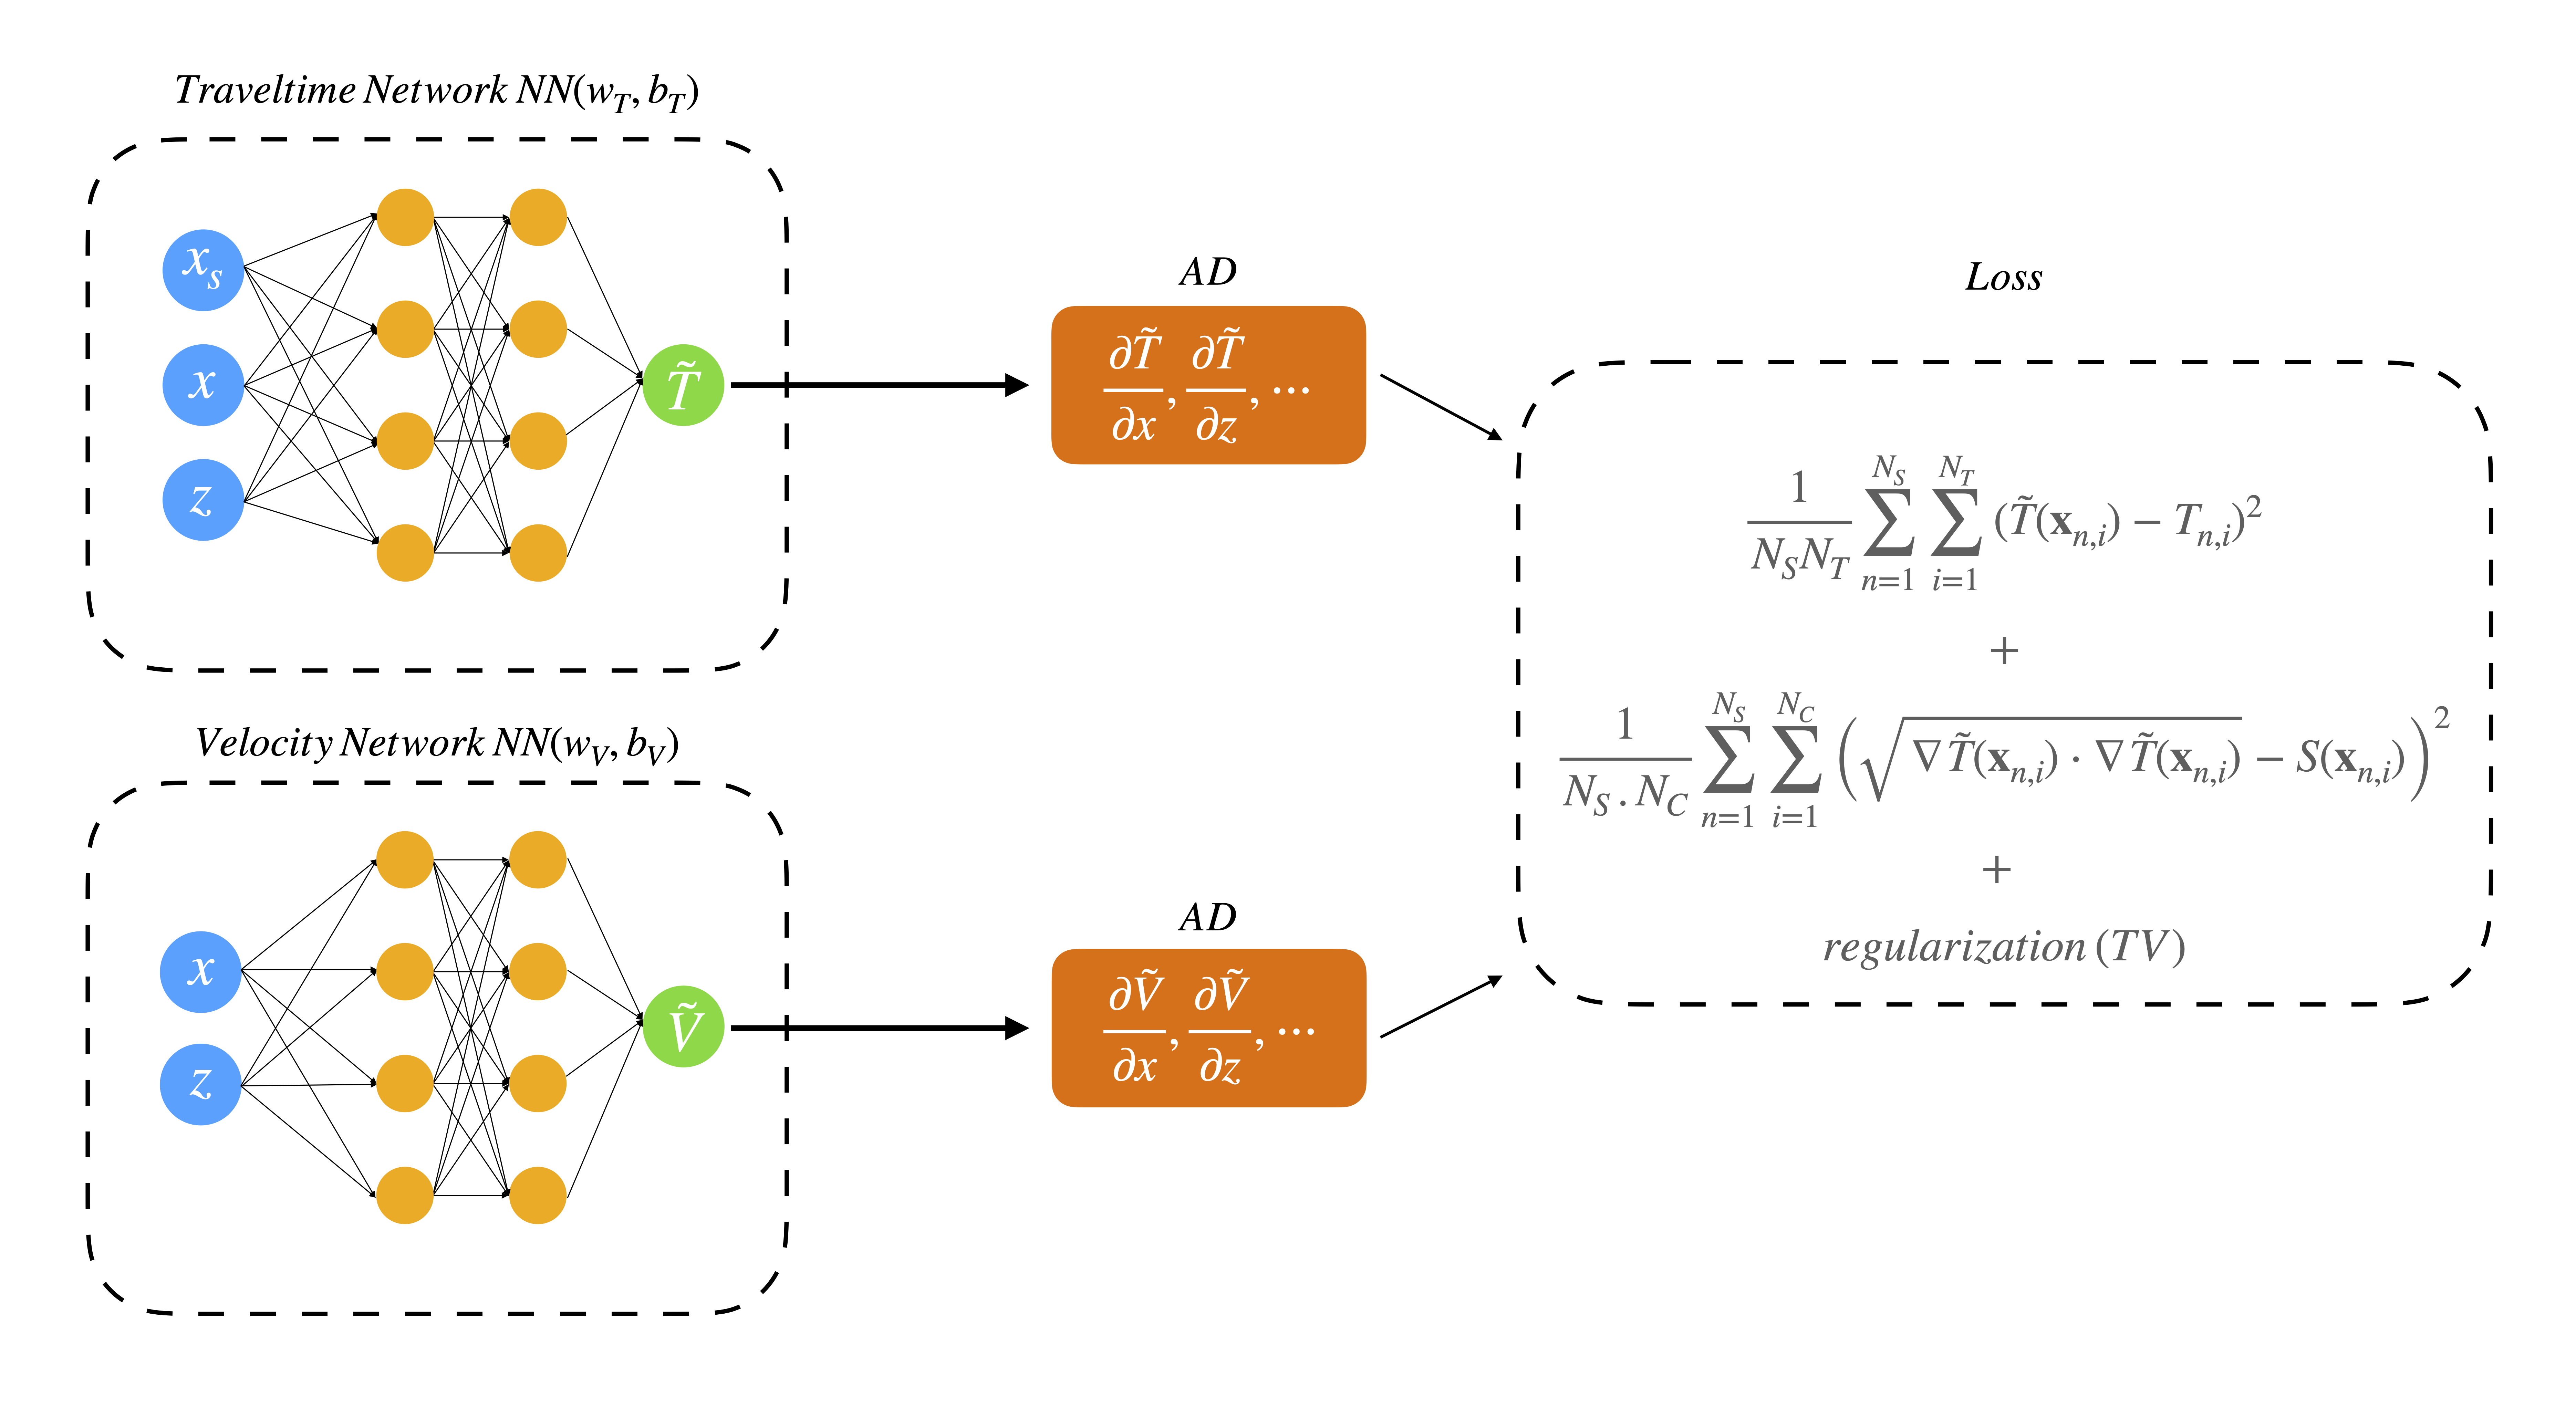
\includegraphics[width=0.9\textwidth]{figures/chap03_pinn_enabled/pinn_schematic} 
 \caption{Illustration of the PINN framework solving for traveltime tomography problem. Two neural networks are used to approximate the traveltime and the velocity. The automatic differentiation is used to calculate the derivatives used in the loss function. Training is performed with a loss function containing the term that minimizes the residuals of the observed times and the network estimated ones, residual of the eikonal equation, and the regularization term.}
 \label{fig:pinn_schematic}
\end{figure}

Hence, the optimization problem seeks to find the optimal network parameters $w_{T}$, $b_{T}$, $w_{V}$, $b_{V}$ such that
\begin{equation}
    \label{eqn:argmin}
    \underset{(w_{T},b_{T},w_{V},b_{V})}{\arg\min} \mathcal{L}(w_{T},b_{T},w_{V},b_{V}).
\end{equation}